
\documentclass[12p]{article}

\usepackage{setspace}
\usepackage[a4paper, total={6in, 8in}]{geometry}
\usepackage{amsmath}
\usepackage{amsthm}
\usepackage{mathtools}
\usepackage{graphicx}
\usepackage{indentfirst}
\usepackage{amssymb}
\usepackage{subfig}
\usepackage{wrapfig}
\usepackage{enumitem}
\usepackage[font=small]{caption}
\usepackage{url}
\usepackage{geometry}
\usepackage[nottoc]{tocbibind}
\usepackage{xspace}
\usepackage{float}

\newtheorem{theorem}{Theorem}[section]
\newtheorem{definition}{Definition}[section]
\DeclarePairedDelimiter\abs{\lvert}{\rvert}
\graphicspath{ {./Images/} }
\onehalfspacing

\begin{document}
  \newgeometry{bottom=0cm, left=2.5cm, right=2.5cm}
  \begin{center}
    {\Huge Documentation}
    \par
    \vspace{40px}
    {\huge Learning to play snake using DDQN agent}
    \par
    \vspace{80px}
    {\LARGE \textbf{András Simon}}
  \end{center}

   
  \restoregeometry
  \newgeometry{bottom=4.3cm, top=3cm}

  \tableofcontents
  \newpage

  \section{Introduction}
    In the snake game we are controlling a snake on a map and try to eat an apple (Figure 1).
    If the snake succesfully eats it,
    then our snake becomes larger by one unit. If the snake hits the
    wall or hits itself, then the game is over. 

    \begin{figure}[h]
    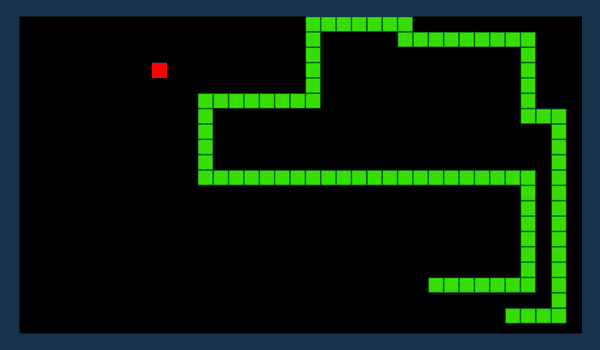
\includegraphics[width=0.7\textwidth]{snake}
    \centering
    \caption{The classic snake game}
    \centering
    \end{figure}

    \par
    In this project a snake-game environment is implemented based on OpenAi AI Gym. 
    Gym is a toolkit for developing and comparing reinforcement learning algorithms.
    For more information see the following website: \textit{https://gym.openai.com/} .
    I created the environment using the description on the GitHub page of the AI Gym on
    \textit{https://github.com/openai/gym/blob/master/docs/creating-environments.md} .
    \par
    The secont part of the project was to create an agent which can learn to play the game.
    The observation from the current state of the environment is a grayscale image, so I used
    a Deep Q Network (DQN) agent on this task. Some results showed that these type of models can solve problems
    like this \cite{atari}.

  \section{Deep reinforcement learning}
    In case of a reinforcement learning problem an agent interacts with it's environment. For every action it takes
    the environment gets a new state and send a reward back to the agent. Based on these experiences the agent can modify
    it's behavior, which is called it's policy. \par
    In case of deep reinforcement learning deep neural networks are used as action-value function approximations. 
    The full introduction to reinforcement learning is out of the scope of this work, but one can learn more about the 
    basic concepts and theory of this field from the introductional book of Richard S. Sutton and Andrew G. Barto \cite{RLintro}.
    \par 
    I want to briefly present in this section the Q-learning, because we will use it later. The following off-policy
    update rule is the base of our implementation:
    \begin{equation}
        Q(s,a) = r + \gamma \max_{a} Q(s', a) ,
    \end{equation}
    where $s$ denotes the current state, $a$ the action, $r$ the reward and $s'$ the new state in a step.
    The $Q$ function is the action-value function, which is a CNN in this case. More precisely
    $Q(s,a)$ is the $a$th output of the model on the $s$ input. $\gamma$ is the discount parameter, a constant.
    The previous formula is used only if
    $s'$ is non-terminal. If $s'$ is terminal, then the formala is changed to
    \begin{equation}
        Q(s,a) = r .
    \end{equation}
    So these $Q$ values will be used as a target to train the network on the state $s$. This target
    is also depends of the network, so it can cause instability. But we will use Double Deep Q Network (DDQN)
    agent istead to stabilize the training. The actual implementation will be described in the later sections. 

  \section{The snake game environment}
    As a parent class the gym.Env class is used from the OpenAi AI Gym toolkit. It has 4 important methods, which
    have to be implamented after the inheritance. For first There is a reset function, which starts a new episode
    and returns the initial observation. In our case it clears the map, creates a random snake and a random apple
    with the given parameters and returns a 2d grayscale image of the game as an numpy array. 
    The image of the game has 80x80 pixles in the test notebook, but it is a 4x4 table. The game is enlarged to contain more pixels.
    The step method takes an
    action as an input and returns a tuple of 4 elements as an output. The first element is the observation of the 
    new state of the game, the second is the reward, the third is a bool variable, which indicates whether the new state
    is terminal or not and finally there is an info object, but i did not used that. The render function shows the game,
    but it's implementation is in a very initial state for now. Finally the close function was not needed to use. 
    After implementing these methods the first test of the env can be performed. This can be found in the environment\_test.py 
    file. \par
    In case of this class one have to declare the observation space and action space too. The observation space is a Box object,
    which abstracts the square shaped inputs, in our case it has 2 dimensions. The action space is discrete, it has 3 values:
    turn left, go ahead and turn right. In this environment the head of the snake is marked with different color (number), than
    the other parts. It simplifies the problem a bit, because we dont have to use 2 images for the imput to follow the motion.
    The apple also has a different color for similar reason. The implementation of the environment can be found in the env folder.
    \par
    The rewrds setting was the following: the snake eat the apple: +1; the snake hits the wall or itself: -1;
    otherwise: -0.01. I used -0.01 for the doing nothing case, beacause i wnated to avoid the going around forever cases. 

  \section{The agent}
    For first i have to mention that, this snake game problem was harder than I expected, and i had to make some experiments to
    achieve good result. The problem can be of course simplified with hand-crafted features, but i wanted to
    use only the image of the game as input.
    The agent which learns to play the game can be used on any 80x80 pixel game with 3 action without modification. In the case of the game
    two images can be quite similar but they can mean very different game states. For example if we consider the
    same snake, but the head and the tail is interchanged. 
    
    \begin{wrapfigure}[25]{r}{0.5\textwidth}
      \vspace{10pt}
      \captionsetup{justification=centering, margin=5pt}
      \begin{center}
      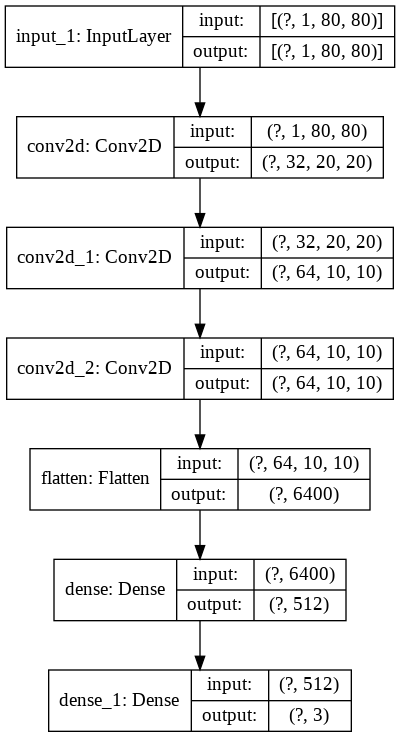
\includegraphics[width=0.4\textwidth]{model}
      \end{center}
      \vspace*{-5mm}
      \caption{The CNN model architecture}
    \end{wrapfigure}

    \par
    The agent is based on the Q-learning, which was introduced in the second section. The agent has 3 important objects: the environment,
    a brain and a memory. The brain contains the models, which can be trained and the memory stores experiences of the game. One
    experience has the form (state, action, reward, new state), which can be used multiple times during the learning. It is very important,
    whithout this the model cannot learn anything. In every step a random batch is choosen from the memory (with 32 samples) and the learning
    is performed on these, instead of the current experience. The brain contains two CNN models with the same structure. The first one is the primary
    model and the second one is the target model. For first I tried the following modification of the Q-learning: train the primary model in every
    step and make prediction using the target network. After some steps load the weights of the primary networks to the target network
    to synchronize them. This was the secont important modification after using the memory. The other changes will cause only small
    improvements compared to this. The main idea behind this is that if the target of the network changes with the network weights in every
    step, than the learning is unstable and may it cannot converge at all. Thats why we have to fix the targets for some time.
    This idea is based on the article of Mnih et al. \cite{2model} and on a useful
    tutorial: \textit{https://jaromiru.com/2016/09/27/lets-make-a-dqn-theory/} \cite{tutorial}. After this worked, I went
    further with double learning, which
    is just a small modification from the previous target model version. In this case we have the following update rule:
    \begin{equation}
        Q_1(s,a) = r + \gamma Q_2(s',argmax_a Q_1(s',a)),
    \end{equation}
    where $Q_1$ is the primary and $Q_2$ is the target network. This new formula means that we make actions using the primary model,
    so we make new experience using that and the evaluation of it's value is performed by the target model as in the previous case.
    So it can also converges well, but it makes the learning curve more smooth. The double learning concept can be fond in two
    articles of Hado van Hasselt, one from 2016 \cite{double1} and an older one from 2010 \cite{double2}.
    \par
    The CNN architecture of the model is not too complicated (Figure 2). This network worked well on this problem, but it is far from optimal.
    One experiment takes a lot of time, aproximately 12 hours, so this hyperparameter adjustment is a possible direction of improvement. 
    \par
    As a learning method I choosed the RMSprop with 0.00025 learning rate. As a loss function as suggested by the previously mentioned tutorial I used the
    Huber loss (Figure 3). It can stabilize the learning in some cases. I used decreasing exploration ratio with 0.1 minimum. 

    \begin{figure}[h]
    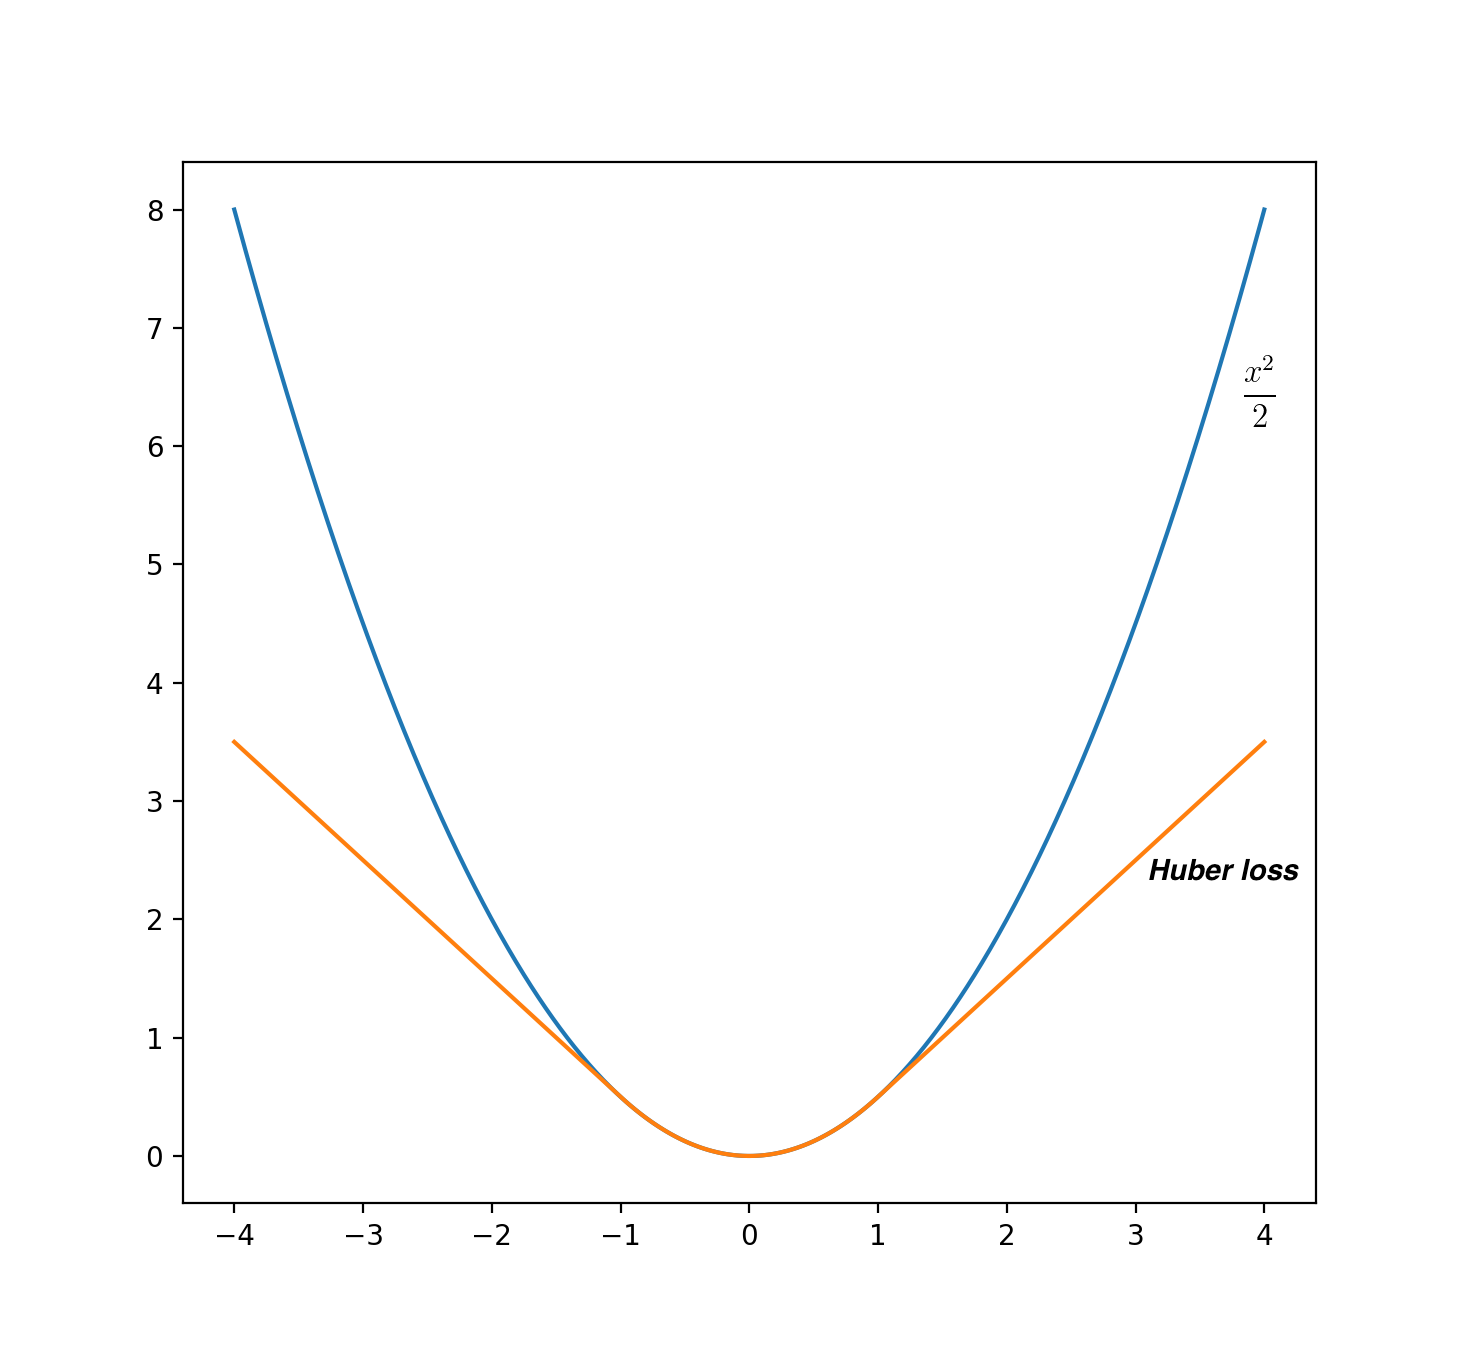
\includegraphics[width=0.7\textwidth]{huber_loss}
    \centering
    \caption{The Huber loss function}
    \centering
    \end{figure}

    \par
    The last improvement what is tried was the prioritized experience replay \cite{PER}, but unfortunately it was too slow to use.

    \section{Test results}
      The test is performed in the DDQN\_agent\_test.ipynb file. The first 1000 episode was played with a random agent to fill the memory.
      After this the DDQN agent was trained for 10000 episodes. The last 100 episode was done with a completely greeady agent (0 epsilon).
      The average reward at the end is above 2, wich means 3 score (-1 is added to the score at the end as reward, because
      of failing). It is below the human level, but it is able to play the game much better than the random agent (Figure 4).

    \begin{figure}[H]
    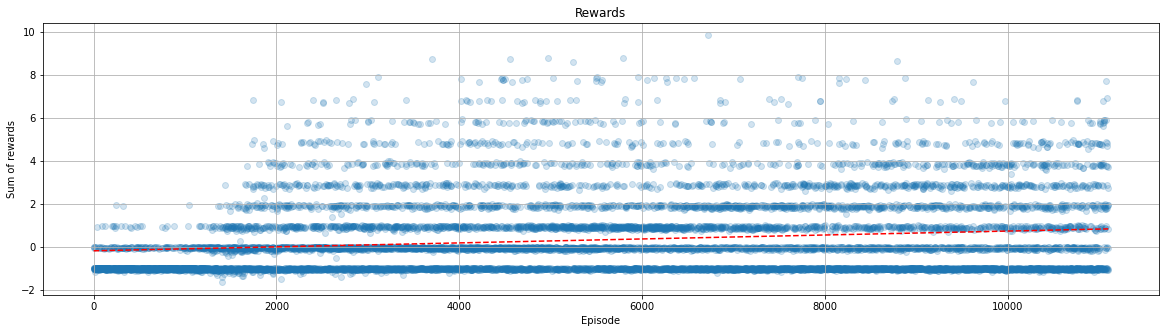
\includegraphics[width=1.1\textwidth]{reward_history}
    \centering
    \caption{The reward history}
    \centering
    \end{figure}

  \begin{thebibliography}{}
    \bibitem{RLintro}
      Richard S. Sutton and Andrew G. Barto.
      Reinforcement Learning An Introduction second edition.

    \bibitem{2model}
      Mnih et al. - Human-level control through deep reinforcement learning, Nature 518, 2015.

    \bibitem{double1}
     Hado van Hasselt, Arthur Guez, David Silver - Deep Reinforcement Learning with Double Q-learning, arXiv:1509.06461, 2016.

    \bibitem{double2}
     Hado van Hasselt - Double Q-learning, Advances in Neural Information Processing Systems, 2010.

    \bibitem{PER}
      Schaul et al. - Prioritized Experience Replay, arXiv:1511.05952, 2015.

    \bibitem{tutorial}
      https://jaromiru.com/2016/09/27/lets-make-a-dqn-theory/ . 2016.

    \bibitem{atari}
      Volodymyr Mnih, et al.
      Playing Atari with Deep Reinforcement Learning. 2013.
  \end{thebibliography}

\end{document}

